% A workaround to allow relative paths in included subfiles
% that are to be compiled separately
% See https://tex.stackexchange.com/questions/153312/subfiles-inside-a-subfile-using-relative-paths
\providecommand{\main}{..}
\documentclass[\main/thesis.tex]{subfiles}

\begin{document}

\chapter{Matrix Multiplication}
\label{cha:matmul}
Matrix multiplication is used extensively in many fields of Science that rely on \gls{hpc}, including several fields within physics~\autocite{krol2014matrix}, biology~\autocite{akutsu2000algorithms} and chemistry~\autocite{weber2015semiempirical}.
It is also possible to simulate quantum computing processes using matrix multiplication~\autocite{zulehner2019matrix}.
Moreover, many neural-network operations are based on matrix-matrix or vector-matrix multiplication~\autocite{rojas1996neural,blue1992training}.

Due to its simple structure, tight loop layout, but potentially long execution time, matrix multiplication is well positioned for improvements through modifications to both software and hardware.
Seminal research, such as that by Goto and van de Geijn~\autocite{goto2008anatomy}, has resulted in high-performance software implementations, including the extensively used linear-algebra libraries EIGEN~\autocite{guennebaud2021eigen} and OpenBLAS~\autocite{xianyi2012model}.
These implementations often outperform na\"ive versions of matrix multiplication by hundreds or thousands of times, turning hours of work into seconds or less.
This speedup is possible through the use of hardware features, such as \gls{simd}, and code transformations, such as loop blocking and data packing.
Understanding matrix multiplication and how it is implemented is critical to achieving these improvements.

\section{Inner and Outer Product}
\label{sec:products}
In the most abstract sense, matrix multiplication is a very simple operation to implement.
As long as each element of $A$ is multiplied with the correct element of $B$ and the result is accumulated to the correct element of $C$, the order in which these operations happen does not matter.
Thus, the simplest implementation of matrix multiplication can be written as in \rlst{basicMatMul}.
\begin{lstlisting}[caption={[Pseudocode for Matrix Multiplication]Pseudocode implementing matrix multiplication as simply as possible.},label=lst:basicMatMul,columns=flexible]
for i=0 to M, j=0 to N, k=0 to D do
  C[i, j] += A[i, k] * B[k, j]
\end{lstlisting}

The order in which the loops are executed does not affect the output of the algorithm on the condition that each combination of $i$, $j$, and $k$ is reached exactly once.
However, mathematically speaking, choosing a certain order for the loops will produce functionality resembling certain common mathematical operations.
A given order for the loops leads to matrix multiplication via the \emph{inner product} (or \emph{dot product}), which is the classic method taught in linear algebra courses, while a different order leads to matrix multiplication via the \emph{outer product}.
While both choices arrive at the same final result, the efficacy with which they arrive can vary significantly, as is discussed later in \rsec{outerKernel} and \rsec{innerKernel}.

\begin{figure}[t]
 \hfill
  \begin{subfigure}{.45\linewidth}
    \centering
    \begin{tikzpicture}[scale=1/2]
      \draw[step=1, shift={(0, 3)}] (0, 0) grid +(4, 1);
      \node at (4.75, 2) {$\times$};
      \draw[step=1, shift={(5.5, 0)}] (0, 0) grid +(1, 4);
      \node at (7.25, 2) {$=$};
      \draw[step=1, shift={(8, 3)}] (0, 0) grid +(1, 1);
      \node at (2, 5) {$A$};
      \node at (6, 5) {$B$};
      \node at (8.5, 5) {$C$};
    \end{tikzpicture}
    \caption{Inner product.}
    \label{fig:innerProduct}
  \end{subfigure}
 \hfill
  \begin{subfigure}{.45\linewidth}
    \centering
    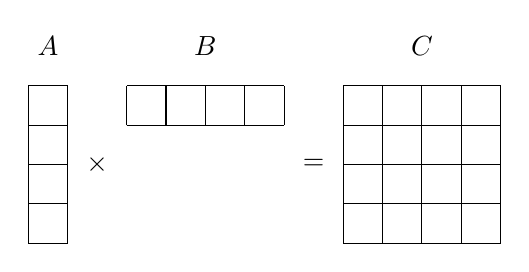
\begin{tikzpicture}[scale=1/2]
      \draw[step=1, shift={(0, 0)}] (0, 0) grid +(1, 4);
      \node at (1.75, 2) {$\times$};
      \draw[step=1, shift={(2.5, 3)}] (0, 0) grid +(4, 1);
      \node at (7.25, 2) {$=$};
      \draw[step=1, shift={(8, 0)}] (0, 0) grid +(4, 4);
      \node at (.5, 5) {$A$};
      \node at (4.5, 5) {$B$};
      \node at (10, 5) {$C$};
    \end{tikzpicture}
  \caption{Outer product (rank-one update).}
    \label{fig:outerProduct}
  \end{subfigure}
  \hfill
  \caption[Matrix-Matrix Computation Styles]{Example matrix-matrix multiplication computation styles.}
  \label{fig:product}
  \vspace{-0.15cm}
\end{figure}

\subsection{The Inner Product}
As taught in the classroom, matrix multiplication can be computed by repeatedly applying the inner product.
The inner product takes two vectors and produces a single scalar value.
Specifically, it is defined as the summation of the pair-wise products of two vectors (\eg $v \cdot w=v_{1}w_{1} + v_{2}w_{2} + \ldots + v_{D}w_{D}$).

Within the context of matrix multiplication, the inner product is used to compute a single cell of $C$ from a row of $A$ and a column of $B$.
More concretely, given the computation \matmul{M}{D}{N}, the inner product computes the cell $c_{i,j}$ by taking the inner product of the $i$th row of $A$ and the $j$th column of $B$ (\rfig{innerProduct}).
In this way, matrix multiplication is composed of one inner product for each cell of $C$.

We can see this process in the following implementation of matrix multiplication:
\begin{lstlisting}[caption={[Basic Matrix Multiplicaion via Inner Product]A basic matrix multiplication via inner product.},label=lst:basicInner,language=C++,columns=flexible,morekeywords=uint64_t,escapechar=|]
for (uint64_t i = 0; i < M; ++i)|\label{innerILoop}|
  for (uint64_t j = 0; j < N; ++j)|\label{innerJLoop}|
      for (uint64_t k = 0; k < D; ++k)|\label{innerKLoop}|
        C[i][j] += A[i][k] * B[k][j];
\end{lstlisting}

Referring back to \rlst{basicMatMul}, the loop order has been concretised to $(i, j, k)$.
In order to implement the mathematical process outlined above, the loops on lines~\ref{innerILoop} and \ref{innerJLoop} of \rlst{basicInner} select the cell from $C$, the row of $A$, and the column of $B$ that will be used.
The innermost loop on line~\ref{innerKLoop} implements the inner product by multiplying elements from the chosen vectors in $A$ and $B$ and then reducing them into the chosen cell of $C$.
One can thus view the implementation in \rlst{basicInner} as a loop over $i$ and $j$ that selects an output cell and repeatedly calls an inner product function.
Therefore, with the choice of loop order $(i, j, k)$, matrix multiplication can be conceptualised as shown in \rlst{basicInnerPseudo}.

\begin{lstlisting}[caption={[Matrix Multiplication Pseudocode Using Inner Product]A basic matrix multiplication via inner product broken into logical concepts.},label=lst:basicInnerPseudo,columns=flexible]
for i=0 to M, j=0 to N do
  C[i, j] = innerProduct(A.row(i), B.column(j))
\end{lstlisting}

\subsection{The Outer Product}
\label{sec:outerProduct}
Matrix multiplication can also be computed through repeated application of the outer product.
In contrast to the inner product, the outer product takes two vectors and produces a matrix.
Specifically, given $v$ and $w$ that have lengths $m$ and $n$ respectively, the outer product produces an $m \times n$ matrix where cell $(i, j)$ is the product of $v_i$ and $w_j$ (\rfig{outerProduct}).

Where, given a vector from $A$ and and a vector from $B$, the inner product fully computes a single cell, the outer product partially computes every cell of the output $C$.
Moreover, each vector of $A$ and $B$ are used only once.
Specifically, given the computation \matmul{M}{D}{N}, matrix multiplication is computed by taking the outer product of column $k$ of $A$ and row $k$ of $B$ and summing the resulting partial matrices.
Because the dimension $D$ dictates both the number of columns in $A$ and the number of rows in $B$, the full matrix multiplication can be computed by performing a total of $D$ outer products.

Using \rlst{basicMatMul} as a model, this process implements matrix multiplication with a loop order of $(k, i, j)$:
\begin{lstlisting}[caption={[Basic Matrix Multiplication via Outer Product]A basic matrix multiplication via outer product.},label=lst:basicOuter,language=C++,columns=flexible,morekeywords=uint64_t,escapechar=|]
for (uint64_t k = 0; k < D; ++k)|\label{outerKLoop}|
  for (uint64_t i = 0; i < M; ++i)|\label{outerILoop}|
    for (uint64_t j = 0; j < N; ++j)|\label{outerJLoop}|
        C[i][j] += A[i][k] * B[k][j];
\end{lstlisting}
Here, the loop on line~\ref{outerKLoop} selects a column from $A$ and a row from $B$ while the loops on lines~\ref{outerILoop} and \ref{outerJLoop} compute the outer product of those vectors.
Thus, in a tranformation similar to the one between \rlst{basicInner} and \rlst{basicInnerPseudo}, \rlst{basicOuter} can be rewritten like so:
\begin{lstlisting}[caption={[Matrix Multiplication Pseudocode Using Outer Product]A basic matrix multiplication via outer product broken into logical concepts.},label=lst:basicOuterPseudo,columns=flexible]
for k=0 to D do
  C += outerProduct(A.column(k), B.row(k))
\end{lstlisting}

\subsubsection{Rank-\texorpdfstring{$r$}{r} Updates}
Some mathematical operations, such as lower-upper factorization, depend on a changing data set, updating a model as new data points are added~\autocite{strange2007efficient}.
This update process is performed by taking a matrix derived from the model and updating it with the outer product of two vectors.
Because the result of the outer product of two vectors, a matrix, will always be of rank one, this operation is called a \emph{rank-one update}.\footnotemark
\footnotetext{All rows and columns are a linear combination of one vector. For example, given $M=xv^T$ all columns in $M$ are a multiple of $x$.}
Matrix multiplication can be computed in the same way by updating a zeroed-out matrix with outer products (the rank-one update), eventually arriving at a fully computed multiplication: $C^1=0; C^{k+1}=C^k+A_{*,k}B_{k,*}$.
With this model, the outer-product matrix multiplication in \rlst{basicOuterPseudo} is rewritten as such:
\begin{lstlisting}[caption={[Matrix Multiplication via Rank-One Update]Matrix multiplication using rank-one update.},label=lst:rankOne,language=C++,columns=flexible,morekeywords=uint64_t]
for k=0 to D do
  rankOneUpdate(C, A.column(k), B.row(k));
\end{lstlisting}

It is not necessary for a complicated model to update itself one data point at a time.
Should, for example, two data points become simultaneously available, two rank-one updates can be performed at the same time.
Updating with two rank-one updates means summing two rank-one matrices; by definition, the summation of two rank-one matrices creates a rank two matrix.\footnotemark
\footnotetext{Given matrices $M_1, M_2 \in \mathcal{R}^{m \times n}$, each rank one, then each matrix has $v_i$, its only basis vector. If $v_1 \ne v_2$, then $M_1+M_2$ has two basis vectors $v_1, v_2$, implying $M_1+M_2$ has rank two.}
Therefore, this operation can now be described as a rank-two update.
This same logic extends to creating updates with greater ranks, giving rise to the rank-$r$ update.\footnotemark
\footnotetext{Common notation is rank-$k$ update; it is changed to rank-$r$ update in this work so as to avoid confusion with $k$ in other uses.}
Revisiting the process in \rlst{rankOne}, this repeated rank-one update process is apparent.
The loop simply performs $D$ rank-one updates, implying that the algorithm can be once again reinterpreted in the form of one rank-$D$ update like so:
\begin{lstlisting}[caption={[Matrix Multiplication Via Rank-\texorpdfstring{$r$}{r} Update]Matrix multiplication using rank-$r$ update.},label=lst:rankR,language=C++,columns=flexible,morekeywords=uint64_t]
// Assumption: A, B are arrays of D vectors
rankRUpdate(C, A, B, /*rank*/ D);
\end{lstlisting}

\section{State of the Art}
Matrix multiplication, as a critical operation in many applications, has been the focus of optimisation research for decades.
Simple insights into matrix multiplication have enabled better data usage, both spatially and temporally.
Contemporary libraries and their overall frameworks are derived from seminal work by Goto and van de Geijn~\autocite{goto2008anatomy}.
More recent work~\autocite{vanzee2015blis,zee2016blis} have improved upon that seminal work, but the overall structure remains the same.
Each of these works aim to improve the portability to new architectures by providing a more modular approach for the micro kernel.
This includes a work by Low \etal which shows that the tuning parameters of the kernels for each architecture can be derived analytically from the architecture specification~\autocite{low2016analytical}.

Goto and van de Geijn's work concludes that matrix multiplication should be implemented in a \emph{layered approach}.
Each of these ``layers'' is typically one or more loops that perform some function before executing the enclosed layer.
It can be convenient to think of each of the upper layers as a function with a nested function call within it.
The innermost layer in this view performs the most basic computation on which the entire operation is built, essentially a small and fast matrix multiplication.
The surrounding layers are concerned with the optimisation of data movement and layout.

Typically, the layered approach consists of two layers:
\begin{enumerate*}[itemjoin={{; }}, itemjoin*={{; and }}, label=\textbf{(\arabic*)}, after={.}]
  \item the blocking strategy responsible for breaking up the computation combined with the packing strategy responsible for optimising data movement between memory and cache as well as data layout within the cache (the \emph{outer kernel} or \emph{macro kernel})
  \item the computation strategy responsible for data movement between cache and register as well as for producing the actual result (the \emph{inner kernel} or \emph{micro kernel})
\end{enumerate*}
This work focuses on building a modular innermost layer and therefore the outer layer is explained only briefly for completeness.

\section{The Outer Kernel}
\label{sec:outerKernel}
There are two operations that are critical to the function of the outer kernel: blocking and packing.
Blocking takes an operation and breaks it into smaller pieces, focusing on computing output in a piecewise manner rather than all at once.
Division is necessary because matrix sizes found in applications are often much larger than what can fit in a cache memory.
Even with this division, the distance between elements within different rows or columns can cause cache conflicts or \gls{tlb} misses.
To increase the spatial locality of accesses, packing takes an operand matrix and makes a copy of a block of data into a smaller buffer where all elements fit in cache simultaneously, allowing faster access times.
Packing can also improve the data access pattern for a more efficient inner kernel, as discussed later in \rsec{blockPack}.

The outer kernel is a delicate dance between blocking and packing.
If the blocking factor is too large (\ie many small blocks) then there is an excessive amount of data movement, requiring packing more often with less reuse of each packed element.
However, when the blocking factor is too small (\ie few large blocks) then blocks no longer fit in cache -- in the worst case, causing page faults -- and packing is ineffective.
The dimensions of the blocking, and therefore the packing, can be determined analytically~\autocite{low2016analytical} and are dependent on the sizes of all levels of the cache present on the target architecture (L1, L2, L3 on modern consumer machines, uncommonly L4).

Goto and van de Geijn address blocking, caching, and \gls{tlb} issues in their work by devising three ways of breaking up both operands and output.
When blocking, each new blocking loop breaks up a single dimension of the matrix multiplication.
Dividing one dimension of a matrix produces a \emph{panel}: a section with one long dimension and one short dimension.
Further dividing a panel produces a section with two short dimensions called a \emph{block}.
Only two of the three dimensions ($M$, $D$, $N$) are blocked while the third is the inner most loop's iteration variable.
This process produces $\binom{3}{2}=3$ different choices for the innermost loops.\footnotemark
\footnotetext{``Three choose two''.}
Different combinations of blocking orders also induce different packing choices that change which of $A$, $B$, and $C$ are packed into L1 and L2 cache.

\subsection{Blocking and Packing for Cache}
\label{sec:blockPack}
The primary concern when blocking and packing for cache is optimising L2 cache bandwidth.
When dimensions $M$ and $N$ are blocked, the innermost loop multiplies a panel by another panel, producing a block.
This breakdown is affiliated with the dot product because it multiplies two panels, which resemble a vector, while producing a block, which resembles a cell.
According to their proposed method, with this breakdown, $C$ will be packed in L2 cache.
Unfortunately, because \gls{gemm} is an accumulating operation (\eg $C \mathrel{+}= AB$), $C$ must be read from cache, accumulated into, and then written back.
When either $A$ or $B$ are packed into L2 cache, as is the case in the other breakdowns, there are only read operations from the L2 cache.
Therefore, the dot product method is less bandwidth efficient because it requires both a read and a write from L2 cache.

An implementer can choose between the remaining two methods (blocking $M$ and $D$ or blocking $D$ and $N$) based on the storage order of $C$.
Within each of these methods, the order in which $D$ and the second dimension are blocked creates two options.
One of these options is considerably better than the other; to demonstrate, without loss of generality, consider the method that blocks $M$ and $D$ and iterates $N$.

Given that $A$ is already packed in L2 cache, the first option, which blocks $D$ then $M$,
\begin{enumerate*}[itemjoin*={{ and }}, label=\textbf{(\arabic*)}, after={.}]
  \item streams $C$ to and from memory
  \item packs $B$ in L1 cache
\end{enumerate*}
Given again that $A$ is packed in L2 cache, the second option, which blocks $M$ followed by $D$,
\begin{enumerate*}[itemjoin*={{ and }}, label=\textbf{(\arabic*)}, after={.}]
  \item streams $B$ from memory
  \item computes $C$ in a temporary in L1 cache which is eventually unpacked and merged with $C$ in memory
\end{enumerate*}
The operations labeled \textbf{(1)} in each option can be assumed to have negligible impact because they can be pipelined with computation.
However, the operations labeled \textbf{(2)} are effectively overhead.
By virtue of the unpacking and merging of $C$ being a more complex operation, the first option is concluded to be superior.
The same logic can be applied to the method which blocks $D$ and $N$ by substituting $N$ for $M$ and swapping which of $A$ and $B$ are packed in L2 cache, arguing that packing $D$ then $N$ is superior.

\subsubsection{Blocking and Packing for Registers}
The dimensions chosen to maximise cache usage are likely to be too large for the registers to handle, thus a further set of loops can be added to block for registers.
These loops only block the pre-packed buffers in memory and do not perform any packing themselves.
Instead, when packing for the cache, the order in which data is packed is modified.
Rather than packing in the same order relative to the original data, data is organised such that these sub-matrix register arguments are contiguous.
Packing in this way results in only a single data copy and allows reads to register for calculation to be contiguous in memory, improving hardware prefetching effects.

\subsubsection{Practicality}
Na\"ive matrix multiplication (\ie \rlst{basicInner}) does not perform blocking nor packing; such a case can be viewed as a ``bare'' inner kernel, without an outer kernel.
Given small matrices as operands, this lack of blocking and packing is often the correct choice.
The overhead resulting from the data movement in the outer kernel is designed to be overshadowed by the speedup gained from improved cache performance.
When input and output data are already small enough to be entirely resident in cache, the effort made to pack and block is shown to be an unnecessary expense.

However, given large matrices, lacking a blocking and packing layer is disastrous for performance.
With sufficiently large matrices, every load will result in a cache miss because the requested data will have been expelled from the cache by a more recent load simply by the pigeonhole principle.
In the worst case, these issues are compounded with \gls{tlb} misses as well.
Therefore, while a single, optimised inner kernel is always critical to performance, it is important for library implementers or compiler designers to consider the size of the data when possible and offer multiple outer-kernel data-management strategies.

\section{The Inner Kernel}
\label{sec:innerKernel}
The inner kernel is focused on maximising performance.
Whether the computation itself has small dimensions or a larger computation has been blocked and packed by an outer kernel, the inner kernel is meant to be as tight and as efficient as possible.
Therefore, the implementation of the inner kernel must consider optimisations such as loop unrolling and instruction rescheduling to improve operation pipelining.
The instruction cache capacity, instruction issue rate, register pressure, and functional unit availability must also be taken into account.
First, however, the product that implements the inner kernel must be chosen.

\subsection{Inner Product vs Outer Product}
\label{sec:productsVs}
Matrix multiplication's inner kernel is implementable through two operations: inner product and outer product.
Both operations arrive at the same destination albeit via different processes.
At the end of the computation, both methods will have performed exactly the same number of multiplications and additions.
In a hypothetical machine with unlimited resources, including vector registers of unlimited length, they would perform the same number of stores and loads.
In such a theoretical framework, at least in terms of computations performed, neither method can be said to be better.
However, in a practical machine, it is impossible to load the entirety of a long row or of a long column into vector registers in order to fully compute a portion of the matrix.

Long dimension lengths make tiling a necessity.
Tiling, as discussed in \rsec{blockPack}, breaks the overall multiplication into smaller, more manageable computations.
As discussed in that same section, on the macro scale, Goto and van de Geijn conclude that a dot-product-based tiling results in more costly data movement, making it a poor choice for the implementation of the outer kernel.

When considering the inner kernel, the dot-product approach also makes poor use of \gls{simd} capabilities.
Computing the dot product requires a horizontal reduction (or tree reduction): the reduction of all the \glspl{lane} of a vector register into a single scalar element.
Computing a partial result in this manner reduces the effectiveness of \gls{simd} by creating a scalar value.
\Gls{simd} was created specifically to alleviate the bottleneck associated with working with scalar values; reverting to scalars should therefore be avoided when possible.
The outer product, on the other hand, uses a vertical reduction (or element-wise reduction) that allows partial products to be accumulated simultaneously in all \glspl{lane} of the destination vector register.

\subsection{Goto's and van de Geijn's Methodology in the Inner Kernel}
\label{sec:gotoInner}

\begin{figure}[t]
  \hfill
  \begin{subfigure}{.45\linewidth}
    \centering
    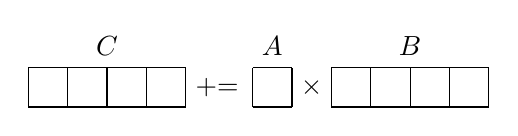
\begin{tikzpicture}[scale=1/2]
      \node[above=.75] at (2, 1) {$C$};
      \draw[shift={(0,0)}] (0,0) grid +(4,1);
      \node at (4.8,.5) {$\mathrel{+}=$};
      \node[above=.75] at (6.2, 1) {$A$};
      \draw[shift={(5.7,0)}] (0,0) grid +(1,1);
      \node at (7.2,.5) {$\times$};
      \node[above=.75] at (9.7, 1) {$B$};
      \draw[shift={(7.7,0)}] (0,0) grid +(4,1);
    \end{tikzpicture}
    \caption{Block times panel.}
    \label{fig:gebpMath}
  \end{subfigure}
  \hfill
  \begin{subfigure}{.45\linewidth}
    \centering
    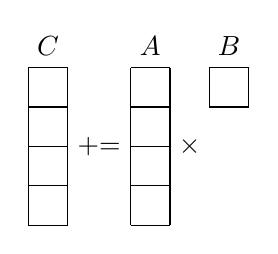
\begin{tikzpicture}[scale=1/2]
      \node[above=.75] at (.5, 4) {$C$};
      \draw[shift={(0,0)}] (0,0) grid +(1,4);
      \node at (1.8,2) {$\mathrel{+}=$};
      \node[above=.75] at (3.1, 4) {$A$};
      \draw[shift={(2.6,0)}] (0,0) grid +(1,4);
      \node at (4.1,2) {$\times$};
      \node[above=.75] at (5.1, 4) {$B$};
      \draw[shift={(4.6,3)}] (0,0) grid +(1,1);
    \end{tikzpicture}
    \caption{Panel times block.}
    \label{fig:gepbMath}
  \end{subfigure}
  \hfill
  \caption[Inner Kernel Implementations, Mathematically]{The two possible implementations for the inner kernel viewed mathematically.}
  \label{fig:gebp}
\end{figure}

\begin{figure}[t]
  \hfill
  \begin{subfigure}{.45\linewidth}
    \centering
    \begin{tikzpicture}
      \draw[step=0.8cm,shift={(0,0)}] (0,0) grid +(.8cm,3.2cm);
      \matrix[matrix of nodes,matrix anchor=south west,inner sep=0pt,minimum height=.8cm,text width=.8cm,align=center,shift={(0,0)}]
      {
        $c_{0,0}$\\
        $c_{0,1}$\\
        $c_{0,2}$\\
        $c_{0,3}$\\
      };
      \node at (1.175cm, 1.6cm) {$\mathrel{+}=$};
      \draw[step=0.8cm,shift={(1.6cm,0)}] (0,0) grid +(.8cm,3.2cm);
      \matrix[matrix of nodes,matrix anchor=south west,inner sep=0pt,minimum height=.8cm,text width=.8cm,align=center,shift={(1.6cm,0)}]
      {
        $a_{0,0}$\\
        $a_{0,0}$\\
        $a_{0,0}$\\
        $a_{0,0}$\\
      };
      \node at (2.75, 1.6cm) {$\times$};
      \draw[step=0.8cm,shift={(3.1cm,0)}] (0,0) grid +(.8cm,3.2cm);
      \matrix[matrix of nodes,matrix anchor=south west,inner sep=0pt,minimum height=.8cm,text width=.8cm,align=center,shift={(3.1cm,0)}]
      {
        $b_{0,0}$\\
        $b_{0,1}$\\
        $b_{0,2}$\\
        $b_{0,3}$\\
      };
    \end{tikzpicture}
    \caption{Block times panel.}
    \label{fig:gebpSimd}
  \end{subfigure}
  \hfill
  \begin{subfigure}{.45\linewidth}
    \centering
    \begin{tikzpicture}
      \draw[step=0.8cm,shift={(0,0)}] (0,0) grid +(.8cm,3.2cm);
      \matrix[matrix of nodes,matrix anchor=south west,inner sep=0pt,minimum height=.8cm,text width=.8cm,align=center,shift={(0,0)}]
      {
        $c_{0,0}$\\
        $c_{1,0}$\\
        $c_{2,0}$\\
        $c_{3,0}$\\
      };
      \node at (1.175cm, 1.6cm) {$\mathrel{+}=$};
      \draw[step=0.8cm,shift={(1.6cm,0)}] (0,0) grid +(.8cm,3.2cm);
      \matrix[matrix of nodes,matrix anchor=south west,inner sep=0pt,minimum height=.8cm,text width=.8cm,align=center,shift={(1.6cm,0)}]
      {
        $a_{0,0}$\\
        $a_{1,0}$\\
        $a_{2,0}$\\
        $a_{3,0}$\\
      };
      \node at (2.75, 1.6cm) {$\times$};
      \draw[step=0.8cm,shift={(3.1cm,0)}] (0,0) grid +(.8cm,3.2cm);
      \matrix[matrix of nodes,matrix anchor=south west,inner sep=0pt,minimum height=.8cm,text width=.8cm,align=center,shift={(3.1cm,0)}]
      {
        $b_{0,0}$\\
        $b_{0,0}$\\
        $b_{0,0}$\\
        $b_{0,0}$\\
      };
    \end{tikzpicture}
    \caption{Panel times block.}
    \label{fig:gepbSimd}
  \end{subfigure}
  \hfill
  \caption[Inner Kernel Implementations, In Register]{The two possible implementations for the inner kernel as computed by using broadcasting and FMA instructions.}
  \label{fig:gepb}
  \vspace{-0.15cm}
\end{figure}

Goto and van de Geijn's methodology continues to be present within the inner kernel of libraries.
As in the outer kernel, rather than implementing matrix multiplication in terms of the dot product, which some \glspl{isa} have directly supported for years\footnotemark, in this methodology matrix multiplication is implemented through the multiplication of a combination of a block and a panel.
\footnotetext{For example, the DPPS or DPPD instructions that were introduced in x86 SSE 4.1 in 2008.}
While for the outer kernel a short dimension is optimally several hundred elements wide and a long dimension is the full extent of one of the matrix dimensions, the inner kernel must operate with registers.
Therefore, a ``short'' dimension is typically a single element and a ``long'' dimension is the length of the vector register.
\rfig{gebpMath} and \rfig{gepbMath} show, in the mathematical sense, what both combinations of block and panel multiplication look like if a vector register can hold four elements.

Next is a discussion of the typical library implementation of these concepts using \gls{simd} techniques in a simple but flawed outer product followed by a presentation of a method to resolve these flaws through an improved version of the outer product.

\subsubsection{Emulating the Outer Product with SIMD Instructions in Libraries}
\label{sec:emulateProduct}
\rfig{gebpSimd} and \rfig{gepbSimd} show how the outer product is emulated using an architecture's \gls{simd} capabilties.
First, the block's single element is \glslink{broadcast}{broadcasted} to each \gls{lane} of a vector register.
The elements of the panel are then loaded into a different vector register.
Once both registers are ready, \ifglsused{fma}{an}{a} \gls{fma} instruction multiplies the two vector registers together and accumulates the result into a third vector register representing a panel in $C$.
This process is more effective than using the dot product because multiple output values are accumulated at the same time in each \gls{lane} of the vector.
However, in a kernel that is supposed to be as tight as possible, cycles are lost to duplicating values.
Furthermore, the kernel should also use resources as effectively as possible, however, the duplicated values use all \glspl{lane} of a vector, effectively reducing a vector register back to a single scalar, nullifying the benefits of \gls{simd}.

\subsubsection{Improving the Design}
\begin{figure}[t]
  \hfill
  \begin{subfigure}{.40\linewidth}
    \centering
    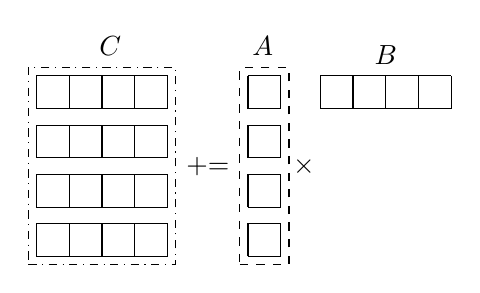
\begin{tikzpicture}[scale=5/12]
      \node[above=.75] at (2, 5.75) {$C$};
      \draw[shift={(-.25,0)}] (0,0) grid +(4,1);
      \draw[shift={(-.25,1.5)}] (0,0) grid +(4,1);
      \draw[shift={(-.25,3)}] (0,0) grid +(4,1);
      \draw[shift={(-.25,4.5)}] (0,0) grid +(4,1);
      \draw[shift={(-.5,-.25)},dashdotted] (0, 0) -- +(4.5, 0) -- +(4.5, 6) -- +(0, 6) -- cycle;
      \node at (4.975,2.75) {$\mathrel{+}=$};
      \node[above=.75] at (6.65, 5.75) {$A$};
      \draw[shift={(6.2,0)}] (0,0) grid +(1,1);
      \draw[shift={(6.2,1.5)}] (0,0) grid +(1,1);
      \draw[shift={(6.2,3)}] (0,0) grid +(1,1);
      \draw[shift={(6.2,4.5)}] (0,0) grid +(1,1);
      \draw[shift={(5.95,-.25)},dashed] (0, 0) -- +(1.5, 0) -- +(1.5, 6) -- +(0, 6) -- cycle;
      \node at (7.9,2.75) {$\times$};
      \node[above=.75] at (10.4, 5.5) {$B$};
      \draw[shift={(8.4,4.5)}] (0,0) grid +(4,1);
    \end{tikzpicture}
    \caption{Extending block times panel.}
    \label{fig:extGebp}
  \end{subfigure}
  \hfill
  \begin{subfigure}{.5\linewidth}
    \centering
    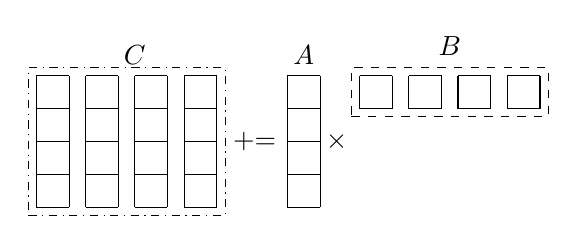
\begin{tikzpicture}[scale=5/12]
      \node[above=.75] at (2.75, 4) {$C$};
      \draw[shift={(-.25,0)}] (0,0) grid +(1,4);
      \draw[shift={(1.25,0)}] (0,0) grid +(1,4);
      \draw[shift={(2.74,0)}] (0,0) grid +(1,4);
      \draw[shift={(4.25,0)}] (0,0) grid +(1,4);
      \draw[shift={(-.5,-.25)},dashdotted] (0, 0) -- +(6, 0) -- +(6, 4.5) -- +(0, 4.5) -- cycle;
      \node at (6.4,2) {$\mathrel{+}=$};
      \node[above=.75] at (7.9, 4) {$A$};
      \draw[shift={(7.4,0)}] (0,0) grid +(1,4);
      \node at (8.9,2) {$\times$};
      \node[above=.75] at (12.35, 4.25) {$B$};
      \draw[shift={(9.6,3)}] (0,0) grid +(1,1);
      \draw[shift={(11.1,3)}] (0,0) grid +(1,1);
      \draw[shift={(12.6,3)}] (0,0) grid +(1,1);
      \draw[shift={(14.1,3)}] (0,0) grid +(1,1);
      \draw[shift={(9.35,2.75)},dashed] (0, 0) -- +(6, 0) -- +(6, 1.5) -- +(0, 1.5) -- cycle;
    \end{tikzpicture}
    \caption{Extending panel times block.}
    \label{fig:extGepb}
  \end{subfigure}
  \hfill
  \caption[Extending Inner Kernels to Outer Product]{Extending Goto and van de Geijn's inner kernel techniques to outer product.}
  \label{fig:extGoto}
\end{figure}

To improve upon this design, it must first be reexamined.
In choosing this method, the implementer is performing a \matmul{1}{1}{n} or \matmul{n}{1}{1} matrix multiplication.
While it is tempting to view this operation as a traditional inner-product, a different point of view can be more beneficial.
Instead, this multiplication can be regarded as a degenerate case of an outer product where one of the operand vector's length is one.
With this understanding, the direction for improvement becomes apparent.
The duplication issue can be resolved by replacing the duplicated values with unique values, extending the outer product's shortened dimension, bringing it closer to \rfig{outerProduct}.
Doing so stacks more of these operations, as shown in \rfig{extGoto}.
A dashed box represents one vector register, with each element therein being a distinct element from the matrix rather than a single \glslink{broadcast}{broadcasted} element.
Given a register that could contain the much larger output data in the dot-dashed boxes, the overhead of broadcasting can be completely removed and the computational throughput of the operation quadrupled.
\rcha{mma} shows how this improvement is possible using \gls{power10}'s \gls{mma}.

\subsection{Implementation}
Having looked at which kernel to implement, discussion can turn towards actual implementation.
As discussed previously, libraries often have kernels handwritten in assembly.
Kernel writers must implement all optimisations by hand.
In doing so, they must review \gls{cpu} properties as well as consider the design of their outer kernel to determine to what degree an optimisation will affect the hardware.
Historically, with great effort, this process has produced excellent results.

Unrolling the kernel to a larger degree allows for greater opportunities in instruction rescheduling as well greater use of available registers.
Computations can be moved closer to loads to enable pipelining as well as interleaved to hide stalls due to occupied functional units.
Future iterations that would load the same data can also be moved such that the values are still in register and can be reused, reducing register pressure and stores.

However, all of these optimisations, and others, are readily available in a compiler, often implemented generically and with great care regarding applicability and benefit analysis.
For example, the kernel can be written in terms of scalars, allowing the compiler to vectorise the kernel automatically.
Automatic vectorisation means obvious optimisations such as using the best available vector load and store instructions as well as unrolling to allow for pipelining of loads.
Less obvious issues are also solved automatically: handling operations that may have dimensions that are not a multiple of vector register automatically creates additional code pathways that vectors at half width, reducing down to scalar computation.
Issues such as new instructions added to an \gls{isa} that are impossible to solve for handwritten kernels without writing an entirely new kernel, are also immediately solved because the compiler knows which architecture to compile for and can use any instruction available on that architecture.
Therefore, a kernel written within the compiler can be written at a higher and more generic level, as in an \gls{ir}, and achieve the same, or better, performance.
It is for this reason that \rcha{method} presents a method built fully within a compiler without a hand-written kernel.

\section{Summary}
This chapter delves in-depth into the intricacies of matrix multiplication, an operation that seems quite simple at first glance.
First to consider are the two main ways in which matrix multiplication can be computed: inner product and outer product.
Both are implemented using the same set of loops and operations and arrive at the same answer, but their performance can vary drastically based on transformations applied when optimising.

The modern approach to optimising matrix multiplication divides the operation into two levels of work.
The first layer, the outer kernel, focuses on efficient manipulation of the memory hierarchy.
This goal is achieved through the use of a blocking and packing strategy derived from seminal work by Goto and van de Geijn.

The inner kernel focuses on optimising the computation of matrix multiplication given the small amount of data provided by the outer kernel at each invocation.
Goto and van de Geijn's influence extends into this layer as well, where they state that the inner product is an inefficient method for computing matrix multiplication.
Despite indications that an outer-product based method is superior, implementation within libraries must rely on emulation via \gls{simd} methods.
However, this method of emulation contains a piece of the outer product in it.
To improve upon the \gls{simd} method, a new hardware extension is required.
\rcha{mma} presents an implementation of that improvement.

\end{document}
